\section{Kiến thức nền tảng}
Trước khi đi vào nghiên cứu bài đề cương luận văn này, một số kiến thức nền tảng cần được nhắc lại như sau.
\subsection{Các kiến thức toán cơ bản}
\subsubsection{Phép nhân tích chập ma trận (convolution)}

Nhân tích chập là phép toán quan trọng trong Xử lý ảnh số và thị giác máy tính, là công cụ chủ yếu để thực hiện các phép tính toán trên ảnh như đạo hàm ảnh, làm trơn ảnh hay trích xuất cạnh.

Trong toán học, tích chập là phép toán trên hai hàm f và g, tạo ra hàm thứ ba là hàm (f*g). Công thức phép tích chập trên miền liên tục một chiều như sau:

\begin{equation}
(f*g)(t) \triangleq \displaystyle \int_{-\infty}^{\infty}f(\tau)g(t-\tau)d\tau
\end{equation}

Đối với trong Xử  lý ảnh, phép tích chập được tính trên miền không gian hai chiều, rời rạc. Công thức tính tích chập trên ảnh f và bộ lọc k (kích thước mxn) tại điểm ảnh vị trí (x,y) với giả sử chỉ số trên bộ lọc được đánh số hàng từ -m/2 -> m/2 và chỉ số cột từ -n/2 -> n/2:




\begin{equation}
    (k*f)(x,y) \triangleq \displaystyle \sum_{u=-m/2}^{m/2}\displaystyle \sum_{v=-n/2}^{n/2}k(u,v)f(x-u,y-v)
\end{equation}

Một phép toán tương tự covolution nhưng không xoay bộ lọc như trên, gọi là correlation (hình \ref {fig:correlation}), công thức như sau:
\begin{equation}
(k*f)(x,y) \triangleq \displaystyle \sum_{u=-m/2}^{m/2}\displaystyle \sum_{v=-n/2}^{n/2}k(u,v)f(x+u,y+v)
\end{equation}


\begin{figure}[!ht]
    \begin{center}
        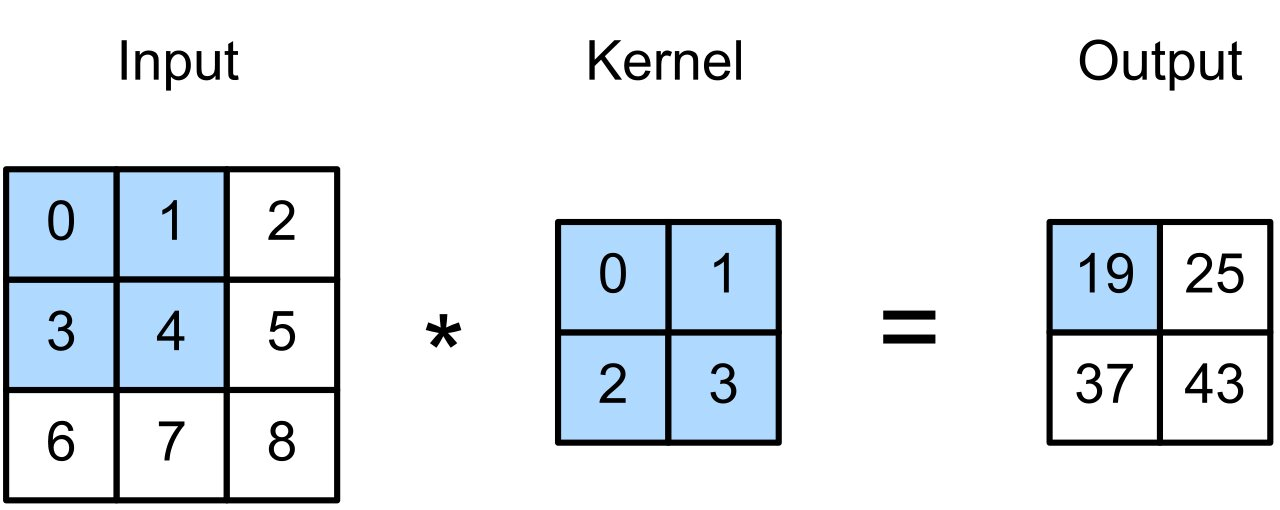
\includegraphics[width=\linewidth]{asset/image/correlation.jpg}
        \caption{Phép correlation.}
        \label{fig:correlation}
    \end{center}
\end{figure}

%chưa nhắc tới strike hay padding gì cả

%graph
\subsubsection{Đồ thị (graph)}

Đồ thị là cấu trúc rời rạc bao gồm các cạnh và các đỉnh được kết nối với nhau thông qua các cạnh đó. Có nhiều loại đồ thị khác nhau, phụ thuộc vào việc có hay không các chiều (direction) của các cạnh, một hay nhiều cạnh cùng kết nối một cặp đỉnh và có chu kì hay không \cite{rosen2012discrete}. 

\textbf{Định nghĩa:}

Một đồ thị G=(V,E) bao gồm V, một tập không rỗng các đỉnh (hay nodes) và E, một tập các cạnh. Mỗi cạnh có một hoặc hai đỉnh liên kết với nó, gọi là endpoints. Một cạnh sẽ kết nối các endpoints của nó \cite{rosen2012discrete}. 

\textbf{Phân loại đồ thị:}

Đồ thị được chia thành nhiều loại dựa vào ba tiêu chí sau:
\begin{enumerate}
\item Đồ thị có hướng hoặc vô hướng.
\item Đơn đồ thị hoặc đa đồ thị.
\item Đồ thị có chu trình hoặc không có chu trình.
\end{enumerate}

Trong Đề cương luận văn này, loại đồ thị được tập trung chủ yếu là đồ thị đơn, vô hướng và không có chu trình. Sau đây ta đi vào cách xây dựng một graph model từ cấu trúc các khớp (joint), xương (bone) của các đối tượng người.

Đối với khung xương người, mỗi khớp sẽ được mô hình hóa thành một đỉnh trong đồ thị, giá trị chứa trong đỉnh là tọa độ của khớp đó trong khung hình (với điểm gốc được định nghĩa tùy vào mục đích bài toán). Mỗi cạnh biểu thị hai đỉnh tương quan với nhau, tức là tồn tại xương giữa hai khớp đó. Độ dài ngắn biểu thị độ xa gần của các khớp. Tùy mục đích mà việc chọn các khớp nào,  hay các xương nào để  mô hình hóa bài toán. Ví dụ với bài toán nhận diện cử chỉ tay, việc tập trung chi tiết các khớp xương ở tay sẽ rất có giá trị, trong khi các khớp xương ở chân và các bộ phận khác sẽ không đóng góp nhiều, do đó không cần định nghĩa trong bài toán.

\begin{figure}[!ht]
    \begin{center}
        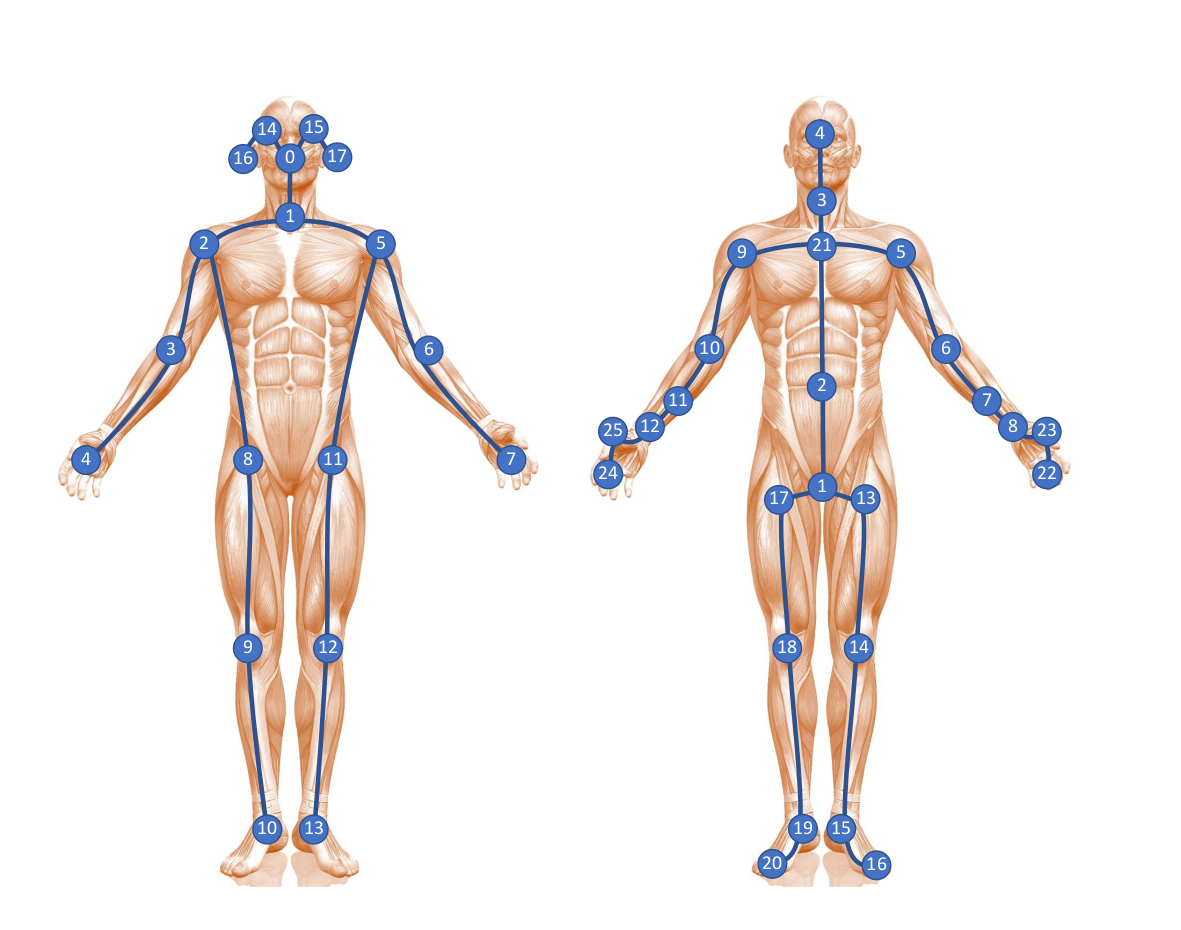
\includegraphics[width=\linewidth]{asset/image/skeleton.png}
        \caption{Graph model cho khung xương người \cite{shi2020skeleton}. }
        \label{fig:skeleton}
    \end{center}
\end{figure}

Trong mô hình thực tế nhóm đang nghiên cứu, tức với mục tiêu nhận diện nhiều loại hành vi của con người, ngoài các cạnh biểu thị các xương sẵn có như hình \ref{fig:skeleton}, nhóm còn định nghĩa thêm các cạnh biểu thị sự tương quan giữa hai đỉnh mà nhóm cho là cần thiết cho mục tiêu bài toán, ví dụ các cạnh giữa hai khớp tay hay giữa khớp tay với khớp chân (hình \ref{fig:morebones}).

\begin{figure}[!ht]
    \begin{center}
        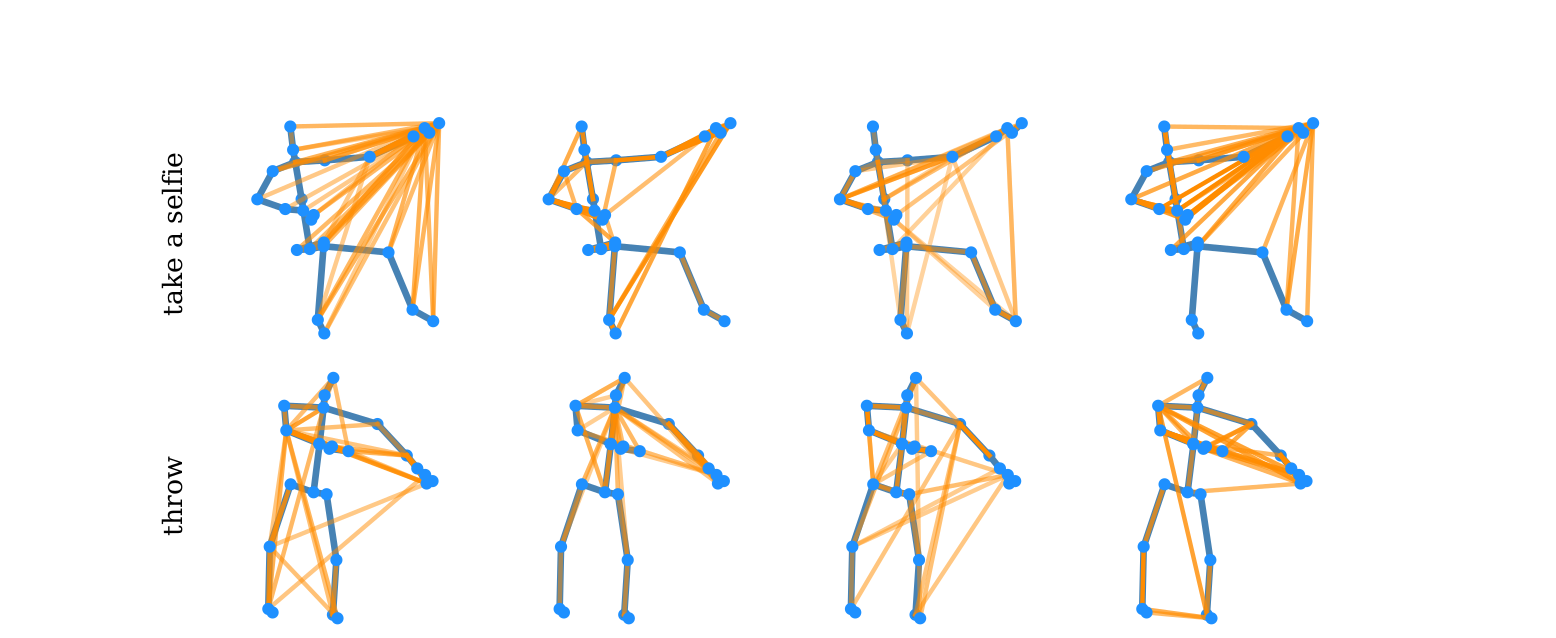
\includegraphics[width=\linewidth]{asset/image/morebones.png}
        \caption{Graph model cho khung xương người với các cạnh bổ sung \cite{shi2020skeleton}. }
        \label{fig:morebones}
    \end{center}
\end{figure}

\subsection{Các kiến thức cơ bản về  Trí tuệ nhân tạo, học máy và học sâu}
\subsubsection{Các kiến thức cơ bản}
%TODO: gradient descent, overfit, underfit, hội tụ, bias, variant, weight, model, loss function, .. tham khảo machinelearningcoban để tránh thiếu sót
%ANN co ban (duoc su dung trng bai: Batch norm, Convolution, resnet, activation: sigmoid, relu,..): embeđing, GCN 
\textbf{Gradient descent - back propagation}

Trong các bài toán tối ưu, việc sử dụng đạo hàm là phương pháp chủ yếu để tìm các điểm cực trị. Việc giải phương trình đạo hàm bằng không đưa ra một tập nghiệm mà tại đó ta chọn ra được các điểm cực trị cần tìm  một cách chính xác. Tuy nhiên với một số bài toán phức tạp, hay các bài toán bất khả vi thì việc tính đạo hàm cũng như giải phương trình đạo hàm bằng không là rất khó, thậm chí là không tồn tại nghiệm. Điều đó đặc biệt đúng trong ngữ cảnh máy học, việc tính chính xác điểm cực trị trong các mô hình học sâu gần như là bất khả thi. Một phương pháp thay thế  để đơn giản hóa việc này, tuy nhiên vẫn giữ được độ chính xác tương đối để đáp ứng nhu cầu bài toán được gọi là \textit{Gradient descent}.

Để  hiểu đươc ý tưởng của \textit{gradient descent}, ta đi vào nghiên cứu ứng dụng của phương pháp  để tìm điểm cực trị của hàm một biến. Xét hàm số $f(x) = \frac{1}{2}(x-1)^2 -2$ có độ thị như hình \ref{fig:grad}, mục tiêu là sử dụng gradient descent để đưa giá trị mà ta cho là nghiệm xấp xỉ $x_t$ về gần với nghiệm thực sự $x^*$. Ta khảo sát đạo hàm $f'(t)$ tại điểm $x_t$ như sau:

\begin{itemize}
    \item nếu $f'(t)>0$ tức $x_t$ lúc này đang ở bên phải của $x^*$, lúc này cần dời vị trí $x_t$ sang bên trái vị trí hiện tại.
    \item ngược lại nếu $f'(t)<0$ tức lúc này $x_t$ đang ở bên trái của $x^*$, và $x_t$ cần được dời về bên phải vị trí hiện tại.
\end{itemize}

Tổng hợp hai trường hợp trên, ta đều phải dời $x_t$ theo chiều ngược lại với giá trị đào hàm tại đó, điều này tương đương với công thức sau:

\begin{equation}
x_(t+1) = x_t - \eta f'(t) 
\end{equation}

Trong đó giá trị $\eta$ thường được gọi là \textit{tốc độ học (learning rate)}. Dấu trừ biểu thị cho việc dời $x_t$ ngược chiều với giá trị đạo hàm. (tham khảo \cite{tiep2018machine}) 
% ******************************************************************************
\begin{figure}[t]
    % caption on side     
    \floatbox[{\capbeside\thisfloatsetup{capbesideposition={right,top},capbesidewidth=6cm}}]{figure}[\FBwidth]
    {\caption{ 
    Khảo sát sự biến thiên của một đa thức bậc hai \cite{tiep2018machine}. 
    }
    \label{fig:grad}}
    { % figure here
    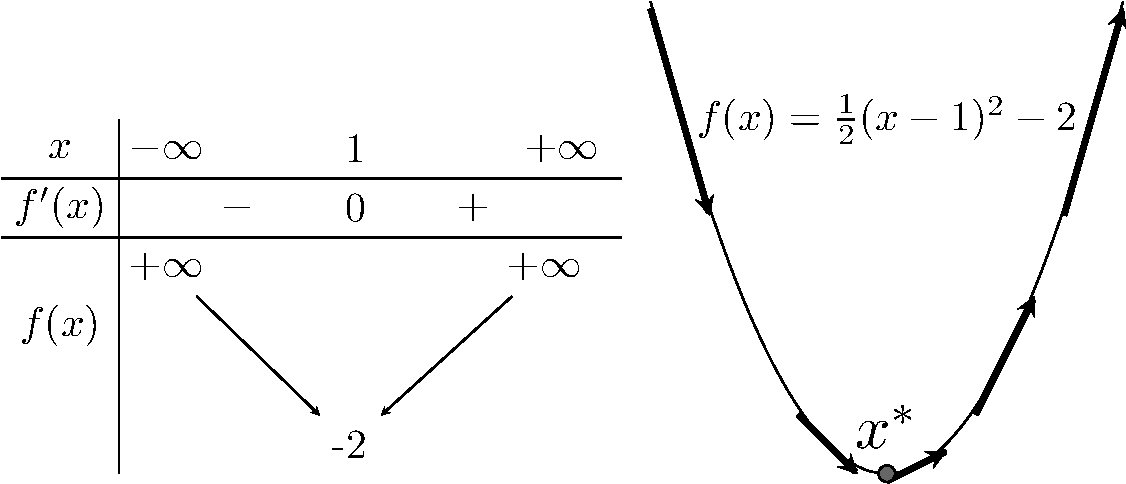
\includegraphics[width=.5\textwidth]{asset/pdf/gradient_descent.pdf}
    }
\end{figure}
% ********

\textbf{Overfitting}

Trong học máy, để một mô hình (model) có thể hoạt động được, ta cần một quá trình giúp mô hình thu nạp kiến thức cần thiết cho việc hoạt động của mô hình, đó được gọi là quá trình học. Quá trình học giúp mô hình có thể cải thiện mức độ khớp (fit) giữa input và output trong tập dữ liệu huấn luyện (training set). Nhưng việc một mô hình có mức độ khớp vượt quá mức cần thiết (overfit) sẽ mang lại hiểu quả không cao, vì lúc này tính tổng quát của mô hình bị giảm đáng kể. Khi một mô hình bị overfit, các tham số của mô hình có xu hướng mô tả chính xác tập dữ liệu huấn luyện nhưng không có khả năng đưa ra phán đoán tốt cho những dữ liệu input mà nó chưa được thấy, đây là điều cần tránh trong học máy.

Trái với hiện tượng này là underfitting, đây là trường hợp mà mô hình chưa được thu nạp đủ kiến thức cho việc đưa ra phán đoán, do đó dẫn tới hiện tượng phán đoán sai trên ngay cả tập dữ liệu huấn luyện và dữ liệu kiểm thử.

Một số phương pháp để giảm hiện tượng overfitting có thể kể tới là validation (hoặc cross-validation nếu tập dữ liệu hạn chế), regularization và early stopping \cite{tiep2018machine}.

\textbf{Variance - bias}

\textbf{Hội tụ}

\textbf{Objective function - loss function}

\textbf{Artificial neural network}

Sau đây sẽ đi qua một vài loại layer quan trọng được sử dụng trong bài toán.
\begin{itemize}
    \item Convolution layer
    \item Graph convolution layer 
    \item BatchNorm layer
    \item Resnet layer
    \item Activation function: sigmoid
    \item Activation function: relu
\end{itemize}

\textbf{Kỹ thuật nhúng -  embedding}

\textbf{Graph Convolution Network}


\subsubsection{Phân loại các phương pháp học}
\textbf{Phân loại phương pháp học}
%TODO: hiện nay có 4 loại học phổ biến: supervised, unsupervised, reinforcement learning, và các phương pháp kết hợp (semi-supervised learning)
\textbf{Phân loại theo ứng dụng}

